% !TeX root = ../main.tex

\section{Introduzione}
Nei precedenti capitoli sono stati introdotti i concetti alla base della cultura DevOps, del ciclo di vita del processo di sviluppo di applicazioni mobile e delle applicazioni multipiattaforma, arrivando a definire un caso di studio industriale. In questo capitolo viene descritto come è stato effettivamente realizzato il sistema per l'automazione del processo di sviluppo nel rispetto dei requisiti e delle specifiche indicate nel capitolo precedente.

In questa fase di realizzazione del sistema di automazione e di implementazione della pipeline viene considerato il progetto base\footnote{\href{https://github.com/paganellif/DevOps-per-applicazioni-mobile-un-caso-di-studio-industriale/tree/3-applicazioni-multipiattaforma/kmm-example}{https://github.com/paganellif/DevOps-per-applicazioni-mobile-un-caso-di-studio-industriale/tree/3-applicazioni-multipiattaforma/kmm-example}} fornito dal plugin KMM\footnote{\href{https://plugins.jetbrains.com/plugin/14936-kotlin-multiplatform-mobile}{https://plugins.jetbrains.com/plugin/14936-kotlin-multiplatform-mobile}} per Android Studio al fine di mantenere il focus sul processo in modo più agnostico possibile rispetto ad una specifica applicazione utilizzatrice come può essere MaggioliEbook, argomento trattato nel capitolo successivo.

\section{Self-Hosted MacOS GitLab Runner}
% runner macos: in azienda non esistono runner macos.. riprendere il problema del fatto che apple obbliga a usare macOS, indicare le possibili soluzioni (runner managed/self-hosted, ecc) e come ho configurato il runner self-hosted
% approfondire tipologie di runner executor in gitlab e perche ho usato l'executor shell
Come anticipato nel capitolo \ref{ch:app-multiplatform} tutta la toolchain per lo sviluppo iOS è disponibile solamente per il sistema operativo macOS, il che implica la necessità di un ambiente macOS anche per l'esecuzione della pipeline, almeno per tutti i task riguardanti l'applicazione iOS. Esistono diversi modi per realizzare un sistema di automazione compatibile con i vincoli imposti da Apple e possono essere suddivisi nelle seguenti categorie:

\begin{itemize}
    \item \textbf{Soluzione completa as-a-Service} - Il grande interesse per l'automazione e lo sviluppo di applicazioni iOS da parte delle aziende ha portato alla nascita di servizi cloud completamente dedicati a questo scopo come ad esempio \textit{Bitrise}\footnote{\href{https://www.bitrise.io/home}{https://www.bitrise.io/home}} e \textit{XCode Cloud}\footnote{\href{https://developer.apple.com/xcode-cloud/}{https://developer.apple.com/xcode-cloud/}}.
    \item \textbf{Runner macOS managed} - Come anticipato nel capitolo \ref{ch:devops} un runner, ovvero il componente che esegue effettivamente i task della nostra pipeline, può essere \textit{managed} o \textit{self-hosted}. Nel caso di un runner managed con sistema operativo macOS si evita lo sforzo di configurare e mantenere un componente importante del sistema di automazione ma si hanno costi elevati: solitamente al consumo di risorse di questa tipologia di runner è applicato un fattore moltiplicativo poco sostenibile in termini di costi. Alcuni esempi di piattaforme con questo modello di business per i runner managed sono GitHub Action\footnote{\href{https://docs.github.com/en/billing/managing-billing-for-github-actions/about-billing-for-github-actions\#minute-multipliers}{https://docs.github.com/en/billing/managing-billing-for-github-actions/about-billing-for-github-actions\#minute-multipliers}} e GitLab CI\footnote{\href{https://docs.gitlab.com/ee/ci/pipelines/cicd\_minutes.html\#additional-costs-on-gitlab-saas}{https://docs.gitlab.com/ee/ci/pipelines/cicd\_minutes.html\#additional-costs-on-gitlab-saas}}.
    \item \textbf{Runner macOS self-hosted} - L'altra tipologia di runner consiste nella installazione del componente su una macchina con sistema operativo macOS che deve essere configurata e mantenuta dall'utilizzatore. In questo caso è possibile utilizzare macchine virtuali as-a-Service, come quelle fornite da AWS\footnote{\href{https://aws.amazon.com/ec2/instance-types/mac/}{https://aws.amazon.com/ec2/instance-types/mac/}} (Amazon Web Services), oppure hardware fisico Apple per installare ed eseguire il runner.
\end{itemize}

Data la disponibilità di tutta la toolchain Android per macOS e il costo nullo in caso di runner self-hosted, è stata scelta quest'ultima tipologia per l'esecuzione dell'intera pipeline.

L'installazione e la configurazione di un runner di questa tipologia può essere più o meno complicata in base alle funzionalità necessarie per il sistema di automazione ed è una procedura chiamata registrazione. Nel caso specifico del caso di studio di questo progetto i principali parametri per la registrazione del runner sono: (\textit{i}) shell executor, (\textit{ii}) token di registrazione al Server CI, (\textit{iii}) cache condivisa e (\textit{iv}) livello di concorrenza.

Definire un executor di tipo \textit{shell} per il runner permette di aprire una nuova shell sulla macchina host per l'esecuzione di ogni job della pipeline e quindi di utilizzare tutti gli strumenti installati sulla stessa macchina.

I seguenti comandi bash\footnote{\href{https://github.com/paganellif/DevOps-per-applicazioni-mobile-un-caso-di-studio-industriale/blob/5-automazione-del-processo-di-sviluppo/setup-gitlab-macos-runner.sh}{https://github.com/paganellif/DevOps-per-applicazioni-mobile-un-caso-di-studio-industriale/blob/5-automazione-del-processo-di-sviluppo/setup-gitlab-macos-runner.sh}} mostrano la procedura di installazione di un runner GitLab macOS self-hosted su una macchina fisica Apple:
\begin{listing}[H]
    \inputminted{bash}{code/macos-runner-setup.sh}
    \caption{Comandi bash per l'installazione, la configurazione e l'avvio di un runner macOS self-hosted}
\end{listing}

Il seguente codice\footnote{\href{https://github.com/paganellif/DevOps-per-applicazioni-mobile-un-caso-di-studio-industriale/blob/5-automazione-del-processo-di-sviluppo/config.toml}{https://github.com/paganellif/DevOps-per-applicazioni-mobile-un-caso-di-studio-industriale/blob/5-automazione-del-processo-di-sviluppo/config.toml}} mostra il contenuto del file di configurazione del runner, generato in seguito alla procedura sopra indicata:

\begin{listing}[H]
    \inputminted{toml}{code/macos-runner-config.toml}
    \caption{File di configurazione (\textit{config.toml}) generato al momento della installazione del runner}
\end{listing}

\section{Modello di branching}
L’utilizzo di un adeguato flusso di lavoro è fondamentale per definire una efficiente automazione CI/CD. Con branching si intende l’utilizzo di uno o più flussi principali dai quali divergono altri flussi per svolgere determinati lavori per poi convergere al loro termine: in base alle modalità di apertura e chiusura di questi flussi si definiscono diversi modelli di branching.

Il modello che si intende utilizzare (fig. \ref{branching}) è basato sul modello di branching GitFlow\footnote{\href{https://www.atlassian.com/it/git/tutorials/comparing-workflows/gitflow-workflow}{https://www.atlassian.com/it/git/tutorials/comparing-workflows/gitflow-workflow}} e prevede tre branch principali:

\begin{itemize}
    \item \textbf{dev} - Flusso principale di sviluppo. Ogni modifica apportata a questo branch corrisponde al rilascio di una nuova versione \textit{alpha} per la validazione interna. E' da questo branch che vengono aperti e chiusi nuovi branch, sia per lo sviluppo di nuove funzionalità (\textit{feature}) che per la risoluzione di bug/patch (\textit{fix}).

    \begin{figure}[H]
        \centering
        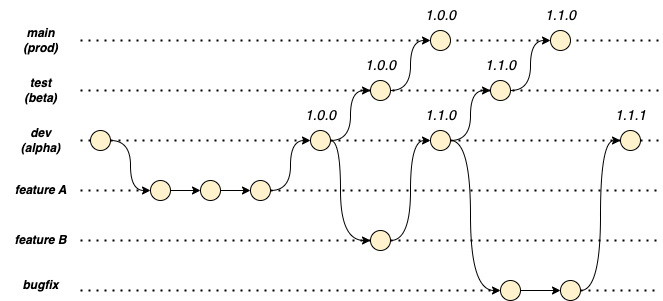
\includegraphics[width=0.65\textwidth]{img/branching-model.png}
        \caption{Esempio di flusso di sviluppo adottando il modello di branching indicato}
        \label{branching}
    \end{figure}
    
    \item \textbf{test} - Branch modificato solamente tramite merge di modifiche provenienti dal branch \textit{dev} con lo scopo di rilasciare una nuova versione \textit{beta} per la validazione esterna.
    \item \textbf{main} - Branch modificato solamente tramite merge di modifiche provenienti dal branch \textit{test} con lo scopo di rilasciare una nuova versione in produzione (\textit{prod}).
\end{itemize}

Grazie ai meccanismi di automazione a supporto della CI/CD fornite dal CI Server si definiscono specifiche regole di attivazione, chiamate \textit{trigger rules}, che permettono di indicare quando uno specifico job deve essere eseguito. Queste regole si basano su eventi che si verificano sul sistema di versionamento come ad esempio commit, tag e merge request. Tramite questa funzionalità è possibile dunque discriminare quali file sono stati modificati e su quale branch per eseguire le operazioni associate come descritto sopra.

\begin{figure}[H]
    \centering
    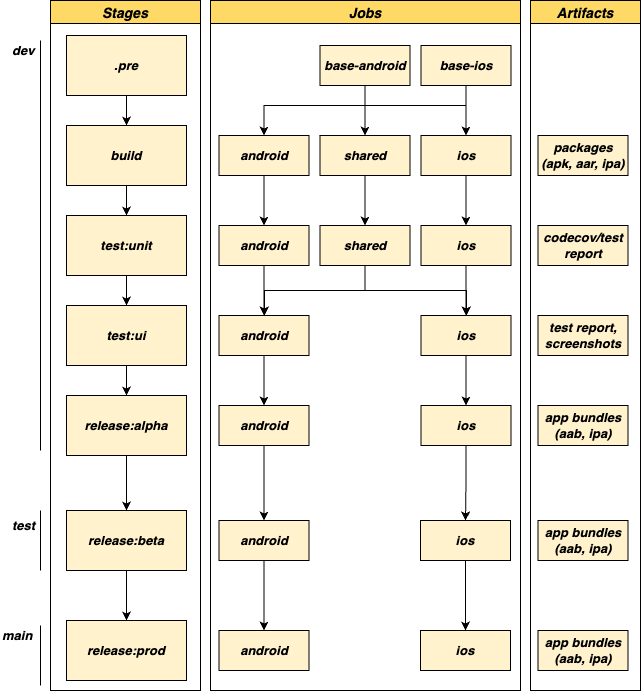
\includegraphics[width=0.85\textwidth]{img/cicd-branch-jobs.png}
    \caption{Stage, job e artefatti associati agli eventi sui branch che compongono l'intera pipeline}
    \label{pipeline-branches}
\end{figure}

\section{Templating}
Uno dei principali vantaggi del meccanismo Pipeline as Code, anticipato nel capitolo \ref{ch:devops}, è la possibilità di utilizzare metodologie per la descrizione delle pipeline simili a quelle utilizzate nella programmazione. Tramite i seguenti strumenti forniti dalla piattaforma GitLab è possibile utilizzare metodologie come ereditarietà e incapsulamento per definire pipeline riutilizzabili:

\begin{itemize}
    \item \textbf{Template} - I file YAML che definiscono una pipeline o sottoparte di essa, possono risiedere in un repository diverso da quello in cui si trova il progetto che la utilizza. In questo modo si definisce una sola volta il flusso base per poterlo successivamente includere e/o estendere negli specifici progetti che necessitano il suo utilizzo.
    \item \textbf{Include} - Definiti i template è necessario includerli all'interno dello specifico progetto per poterli utilizzare effettivamente.
    \item \textbf{Extend} - Definendo lo script del job padre in modo parametrico è possibile pilotarne il comportamento tramite la definizione di variabili d'ambiente nel job figlio. Questa funzionalità è una alternativa alle \textit{anchors} fornite nativamente da YAML ma più flessibile e leggibile.
    \item \textbf{Hidden Jobs} - I job definiti con un punto all'inizio del nome non vengono considerati dal linter GitLab e quindi esclusi dalla esecuzione tramite il runner. Definendo job "nascosti" è possibile definire tutti quegli aspetti comuni e parametrizzabili da estendere con altri job.
\end{itemize}

Il seguente codice\footnote{\href{https://github.com/paganellif/DevOps-per-applicazioni-mobile-un-caso-di-studio-industriale/blob/5-automazione-del-processo-di-sviluppo/kmm-templates/kmm-base.yml}{https://github.com/paganellif/DevOps-per-applicazioni-mobile-un-caso-di-studio-industriale/blob/5-automazione-del-processo-di-sviluppo/kmm-templates/kmm-base.yml}} mostra il job padre di ogni job dedicato alla applicazione iOS, definito come hidden job parametrico: ogni job figlio dovrà estendere questo job e definirne dei valori per le variabili d'ambiente.

\begin{listing}[H]
    \inputminted{yaml}{code/base-ios-job.yaml}
    \caption{Hidden Job parametrico per i job iOS}
\end{listing}

Considerando la composizione della pipeline obiettivo (fig. \ref{pipeline-branches}) una possibile organizzazione ottimale è la definizione di più template\footnote{\href{https://github.com/paganellif/DevOps-per-applicazioni-mobile-un-caso-di-studio-industriale/tree/5-automazione-del-processo-di-sviluppo/kmm-templates}{https://github.com/paganellif/DevOps-per-applicazioni-mobile-un-caso-di-studio-industriale/tree/5-automazione-del-processo-di-sviluppo/kmm-templates}}, uno per ogni fase del processo, in modo da poter importare anche solamente una sottoparte della pipeline:

\begin{itemize}
    \item \textbf{kmm-base} - Definisce tutte le configurazioni di base della pipeline come ad esempio gli stage, le variabili d'ambiente globali e i job di pre-configurazione.
    \item \textbf{kmm-build} - Definisce i job relativi alla fase di compilazione e packaging.
    \item \textbf{kmm-test} - Definisce i job per le fasi di unit testing e ui testing.
    \item \textbf{kmm-analysis} - Definisce i job per le fasi di analisi statica del codice, analisi delle dipendenze e integrazione con SonarQube.
    \item \textbf{kmm-release} - Definisce i job utili alla stabilizzazione e rilascio delle applicazioni (alpha-beta-prod).
\end{itemize}

Realizzati i template è possibile utilizzarli tramite inclusione remota come nel seguente codice\footnote{\href{https://github.com/paganellif/DevOps-per-applicazioni-mobile-un-caso-di-studio-industriale/blob/5-automazione-del-processo-di-sviluppo/.gitlab-ci.yml}{https://github.com/paganellif/DevOps-per-applicazioni-mobile-un-caso-di-studio-industriale/blob/5-automazione-del-processo-di-sviluppo/.gitlab-ci.yml}} d'esempio:

\begin{listing}[H]
    \inputminted{yaml}{code/template-usage.yaml}
    \caption{Esempio d'utilizzo dei template GitLab da repository remoto}
\end{listing}

\section{Continuous Integration}
\subsection{Pre}
Molti dei passi che compongono una pipeline utilizzano tipicamente gli stessi tools e le stesse configurazioni per svolgere task diversi. Ad esempio la compilazione del codice e l'esecuzione degli unit test per una applicazione Java utilizzano in entrambi i casi la stessa JDK\footnote{Java Development Kit}, lo stesso tool di build automation e devono essere scaricate le stesse dipendenze di progetto dal package manager di riferimento.

Utilizzando meccanismi di caching e passaggio di artefatti tra i vari job è possibile eseguire tutti quei task di configurazione una sola volta all'inizio della pipeline risparmiando tempo e risorse in tutte le fasi successive.

Nel caso della pipeline progettata per lo sviluppo di applicazioni multipiattaforma con KMM è necessario eseguire i seguenti task di configurazione iniziale:
\begin{itemize}
    \item Configurazione dell'ambiente per lo sviluppo Kotlin tramite l'installazione e il caching degli SDK e del sotto-compilatore \textit{Kotlin/Native}\footnote{\href{https://kotlinlang.org/docs/native-improving-compilation-time.html\#general-recommendations}{https://kotlinlang.org/docs/native-improving-compilation-time.html\#general-recommendations}} per lo sviluppo multipiattaforma.
    \item Configurazione dell'ambiente per lo sviluppo Android tramite l'installazione del SDK Android target e dei vari tools necessari tramite \textit{sdkmanager}\footnote{\href{https://developer.android.com/studio/command-line/sdkmanager}{https://developer.android.com/studio/command-line/sdkmanager}}.
    \item Configurazione dell'ambiente per lo sviluppo iOS tramite impostazione di XCode e CLI Developer Tools.
    \item Installazione e caching di tutte le dipendenze dei vari moduli.
    \item Configurazione delle chiavi per l'autenticazione ai servizi cloud forniti da Google e Apple.
\end{itemize}

Il seguente codice\footnote{\href{https://github.com/paganellif/DevOps-per-applicazioni-mobile-un-caso-di-studio-industriale/blob/5-automazione-del-processo-di-sviluppo/kmm-templates/kmm-base.yml}{https://github.com/paganellif/DevOps-per-applicazioni-mobile-un-caso-di-studio-industriale/blob/5-automazione-del-processo-di-sviluppo/kmm-templates/kmm-base.yml}} mostra il job di pre-configurazione per tutti i job successivi riguardanti la piattaforma Android:

\begin{listing}[H]
    \inputminted{yaml}{code/pre-android-job.yaml}
    \caption{Job di pre-configurazione Android}
\end{listing}

\subsection{Build e Packaging}
Tipicamente la fase di integrazione continua inizia con la verifica della corretta compilazione del codice sorgente. La compilazione rappresenta un vincolo essenziale per tutte le successive fasi e per questo è definita come fase bloccante: in caso di compilazione fallita la pipeline termina senza procedere con le fasi successive definite.

Nel caso dello sviluppo di applicazioni mobile, per lo stage iniziale di build la pratica più diffusa è quella di validare sia la compilazione del codice che la pacchettizzazione della applicazione nei formati richiesti dalle piattaforme target. Dato il funzionamento di una applicazione KMM (Capitolo \ref{ch:app-multiplatform}) è necessario compilare il codice del modulo condiviso \textit{shared} e quello specifico delle piattaforme Android e iOS e impacchettarlo negli artefatti che verranno passati in input alla fase di delivery, rispettivamente aar\footnote{Android Library}, aab e ipa.

Il seguente codice\footnote{\href{https://github.com/paganellif/DevOps-per-applicazioni-mobile-un-caso-di-studio-industriale/blob/5-automazione-del-processo-di-sviluppo/kmm-templates/kmm-build.yml}{https://github.com/paganellif/DevOps-per-applicazioni-mobile-un-caso-di-studio-industriale/blob/5-automazione-del-processo-di-sviluppo/kmm-templates/kmm-build.yml}} mostra il template che definisce il job base di compilazione e pacchettizzazione della applicazione Android tramite l'utilizzo combinato di fastlane e gradle:
\begin{listing}[H]
    \inputminted{yaml}{code/build-job.yaml}
    \caption{Pipeline job dedicato alla compilazione e pacchettizzazione della applicazione Android}
\end{listing}

\subsection{Testing}
Terminato con successo lo stage di verifica della compilazione e pacchettizzazione del codice segue la fase di test, per la quale si distinguono due tipologie principali di testing: la prima con lo scopo di validare la logica applicativa, chiamata \textit{Unit Testing} e la seconda per la validazione dell'interfaccia grafica, chiamata \textit{UI Testing}.

Quando si parla di testing in ambito mobile ci si riferisce tipicamente alla specifica tipologia di test chiamata \textit{Instrumented Testing}, dove è necessario realizzare un progetto di test apposito in modo da installare e testare la applicazione in un ambiente simulato come per esempio quello fornito dagli emulatori~\cite{darwin2011android}. In realtà l'instrumentazione di una applicazione è necessaria solamente per quei test dove vengono richiamate le API dello specifico SDK della piattaforma target, come nel caso della UI testing.

\subsubsection*{Unit Testing}
Con unit testing si intende l’attività di verifica di certe porzioni (unità) del codice ed è implementato tipicamente utilizzando librerie predisposte per ciascun linguaggio di programmazione. I movimenti Agile e TDD\footnote{Test Driven Development} incoraggiano la scrittura di unit test automatizzati, i quali dovrebbero essere scritti prima dello sviluppo effettivo del codice~\cite{martin2017clean}.

Nonostante la struttura di una applicazione KMM contenga tutta la logica applicativa nel modulo condiviso è necessario eseguire test anche su porzioni di codice specifico delle piattaforme. Le librerie utilizzate per questo scopo sono:

\begin{itemize}
    \item \textbf{JUnit}\footnote{\href{https://junit.org/junit5/}{https://junit.org/junit5/}} - Framework di unit testing per il linguaggio di programmazione Java, utilizzato nel caso di studio per il testing unitario del modulo condiviso e della applicazione Android.
    \item \textbf{XCTest}\footnote{\href{https://developer.apple.com/documentation/xctest}{https://developer.apple.com/documentation/xctest}} - Framework standard di testing per progetti XCode, tra cui unit testing di codice Swift/Objective-C.
\end{itemize}

\subsubsection*{UI Testing}
Analogamente agli unit test, dove si verifica l'integrità della logica applicativa a fronte di una modifica del codice sorgente, negli UI test si verifica l'integrità della interfaccia grafica e dell'esperienza utente. In questa sotto-fase di testing sono coinvolti solamente i moduli che implementano la U e vengono testati tramite le seguenti librerie:

\begin{itemize}
    \item \textbf{Espresso} - Framework standard per lo UI testing di applicazioni Android.
    \item \textbf{XCTest} - Framework standard di testing per progetti XCode, tra cui ui testing di applicazioni iOS (XCUI\footnote{\href{https://developer.apple.com/documentation/xctest/user\_interface\_tests}{https://developer.apple.com/documentation/xctest/user\_interface\_tests}}).
\end{itemize}

Questa specifica fase della pipeline è l'unica che richiede la simulazione degli ambienti tramite l'emulazione dei dispositivi. Per poter eseguire un emulatore di qualsiasi tipo attraverso un sistema di automazione è necessario considerare alcuni aspetti fondamentali come: (\textit{i}) modalità \textit{headless} per l'esecuzione senza interfaccia grafica e (\textit{ii}) accesso concorrente alle risorse del sistema host sul quale eseguono.

Dato il consumo di risorse elevato degli emulatori solitamente si tende ad eseguire in questa fase anche altre operazioni che possono essere automatizzate e che necessitano di un emulatore. Combinando l'esecuzione dei test sulla interfaccia grafica con la cattura delle schermate è possibile ottimizzare il flusso di lavoro e ottenere direttamente dal sistema di automazione gli screenshot desiderati. Con la diffusione di questa pratica sono stati creati tool appositi, come quelli forniti dallo strumento Fastlane adottato:

\begin{itemize}
    \item \textbf{Screengrab}\footnote{\href{https://docs.fastlane.tools/actions/screengrab/}{https://docs.fastlane.tools/actions/screengrab/}} - Tool specifico per Android che richiede la definizione di appositi test utilizzando (\textit{i}) Espresso per navigare nella applicazione in esecuzione e (\textit{ii}) Screengrab\footnote{\href{https://mvnrepository.com/artifact/tools.fastlane/screengrab}{https://mvnrepository.com/artifact/tools.fastlane/screengrab}} per la cattura delle schermate.
    \item \textbf{Snapshot}\footnote{\href{https://docs.fastlane.tools/actions/snapshot/}{https://docs.fastlane.tools/actions/snapshot/}} - Tool specifico per iOS che genera codice\footnote{\href{https://github.com/paganellif/DevOps-per-applicazioni-mobile-un-caso-di-studio-industriale/blob/5-automazione-del-processo-di-sviluppo/SnapshotHelper.swift}{https://github.com/paganellif/DevOps-per-applicazioni-mobile-un-caso-di-studio-industriale/blob/5-automazione-del-processo-di-sviluppo/SnapshotHelper.swift}} Swift in grado di sfruttare XCTest per la navigazione della applicazione e la cattura delle schermate.
\end{itemize}

Il seguente job\footnote{\href{https://github.com/paganellif/DevOps-per-applicazioni-mobile-un-caso-di-studio-industriale/blob/5-automazione-del-processo-di-sviluppo/kmm-templates/kmm-test.yml}{https://github.com/paganellif/DevOps-per-applicazioni-mobile-un-caso-di-studio-industriale/blob/5-automazione-del-processo-di-sviluppo/kmm-templates/kmm-test.yml}} base mostra la strategia utilizzata nel caso di studio per avviare un emulatore Android, eseguire i test sulla interfaccia grafica e restituire, come artefatto, le immagini delle schermate catturate:
\begin{listing}[H]
    \inputminted{yaml}{code/base-ui-test-android.yaml}
    \caption{Job base Android dedicato al testing della interfaccia grafica e alla cattura delle schermate}
\end{listing}

\subsection{Dependency Management}

\section{Continuous Delivery}

\subsection{Alpha/Beta Release}

\section{Continuous Inspection}
% progettazione e implementazione analisi
